\chapter{模型评估}

\section{模型评估标准}
我们选取了准确率,KS统计量以及AUC作为三种模型的评估标准,为了理解这三种评估标准,首先介绍一下分类问题
的最终可能几种结果,见表\ref{tab:roc}。

\begin{table}[htbp]
  \centering
    \begin{tabular}{rrr}
    \toprule
          & \multicolumn{2}{c}{真实值} \\
    \midrule
    \multicolumn{1}{c}{\multirow{2}[0]{*}{预测值}} & 真阳(TP) & 伪阳(FP) \\
    \multicolumn{1}{c}{} & 伪阴(FN) & 真阴(TN) \\
    \bottomrule
    \end{tabular}%
  \label{tab:roc}%
\end{table}%

其中准确率等于$\frac{TP+TN}{TP+FP+FN+TN}$,KS统计量以及AUC是通过接受者操作特征曲线(ROC曲线)得到的。
ROC曲线的横坐标为$False Positive Rate = \frac{FP}{FP+TN}$,纵坐标为$TRUE Positive Rate = \frac{TP}{TP+FN}$
(见如\ref{fig:roc})。其中KS统计量为纵坐标与横坐标差值的最大值,AUC为ROC曲线与横坐标所围的面积,其理想值
为1。

\begin{figure}
\centering
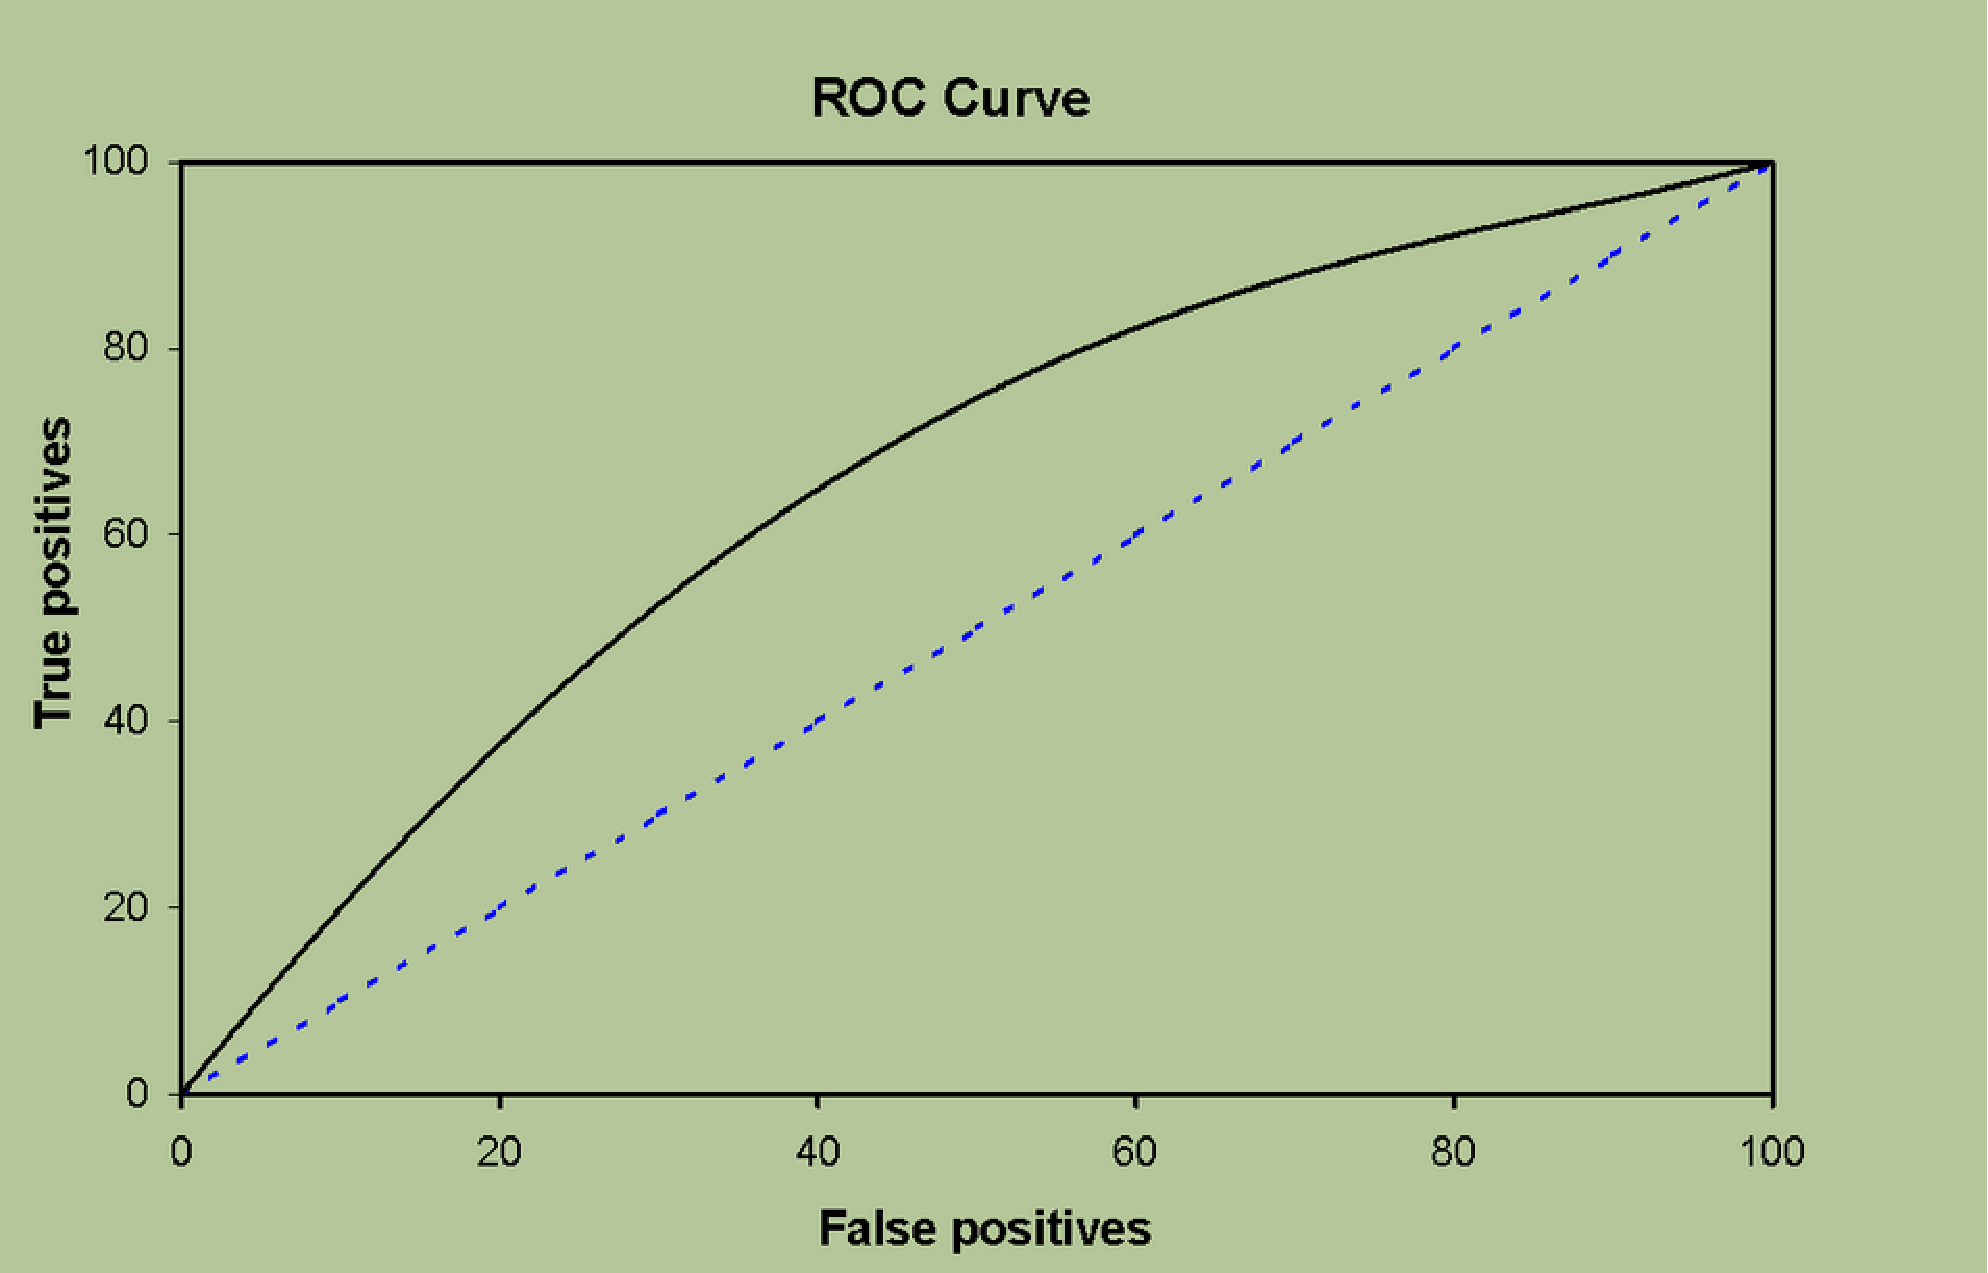
\includegraphics[width=0.8\linewidth]{roc.pdf}
\caption{\label{fig:roc}接受者操作特征曲线(ROC)}
\end{figure}

\section{模型评估结果}
\subsection{German Credit}
以German Credit为训练数据,得到以下结果:

\begin{figure}
\centering
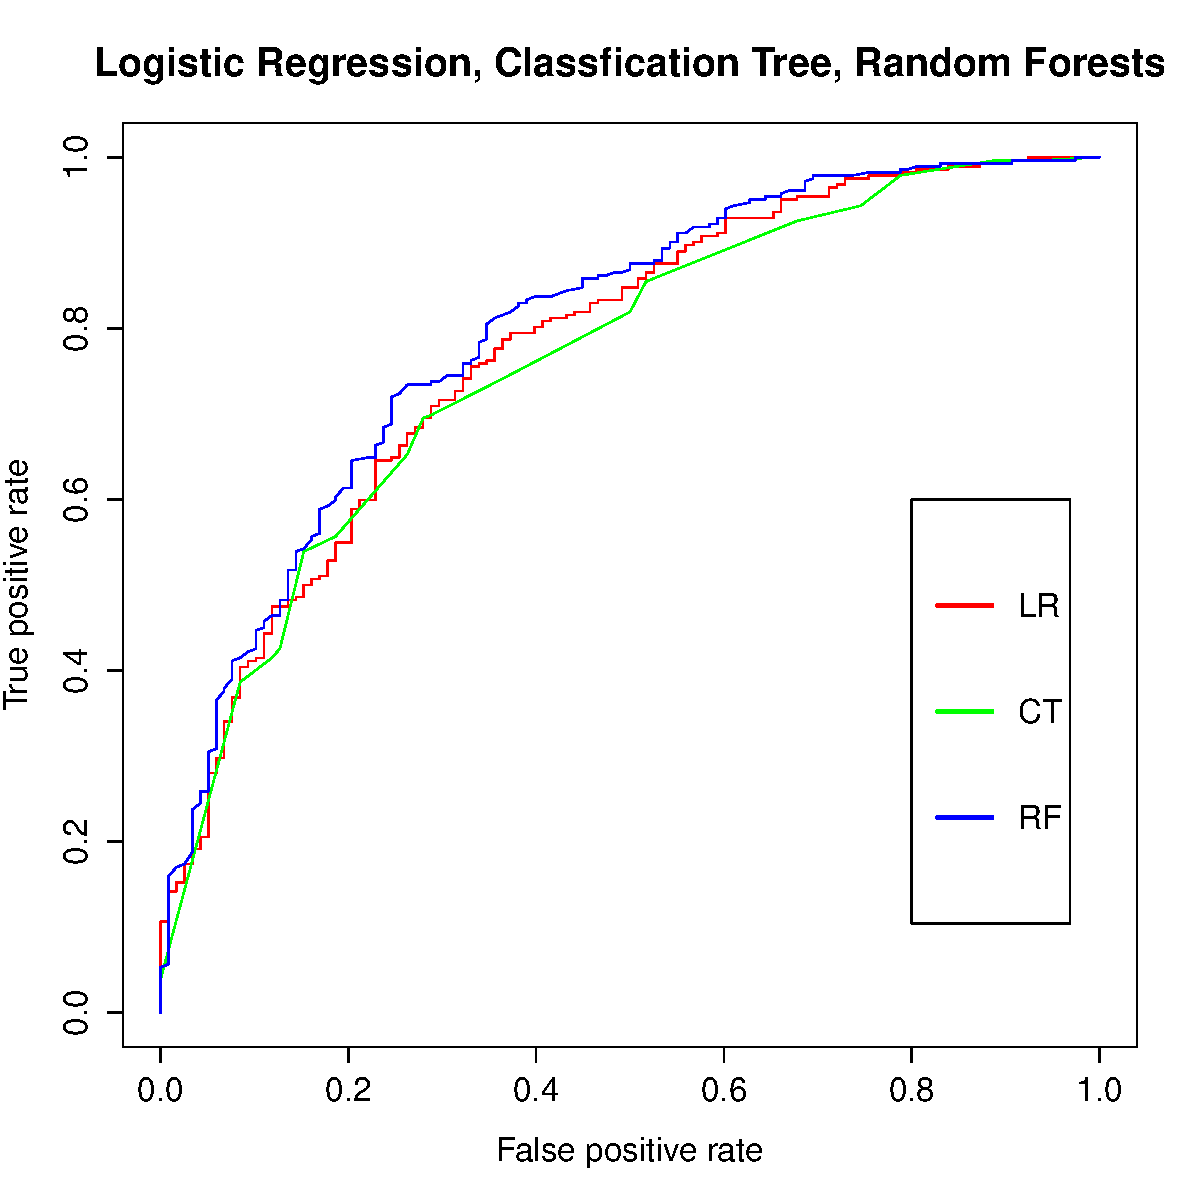
\includegraphics[width=0.8\linewidth]{roc1.pdf}
\caption{\label{fig:roc1}German Credit - ROC}
\end{figure}

\begin{table}[htbp]
  \centering
  \caption{German Credit}
    \begin{tabular}{lllll}
    \toprule
    Model & KS  & AUC & Accuracy  & Cutoff \\
    \midrule
    LR & 0.425 & 0.776 & 0.773 & 0.421 \\
    CT & 0.415 & 0.762 & 0.753 & 0.250 \\
    RF & 0.474 & 0.798 & 0.780  & 0.472 \\
    \bottomrule
    \end{tabular}%
  \label{tab:roc1}%
\end{table}%

\subsection{Give Me Some Credit}
以Give Me Some Credit为训练数据,得到以下结果:
\begin{figure}
\centering
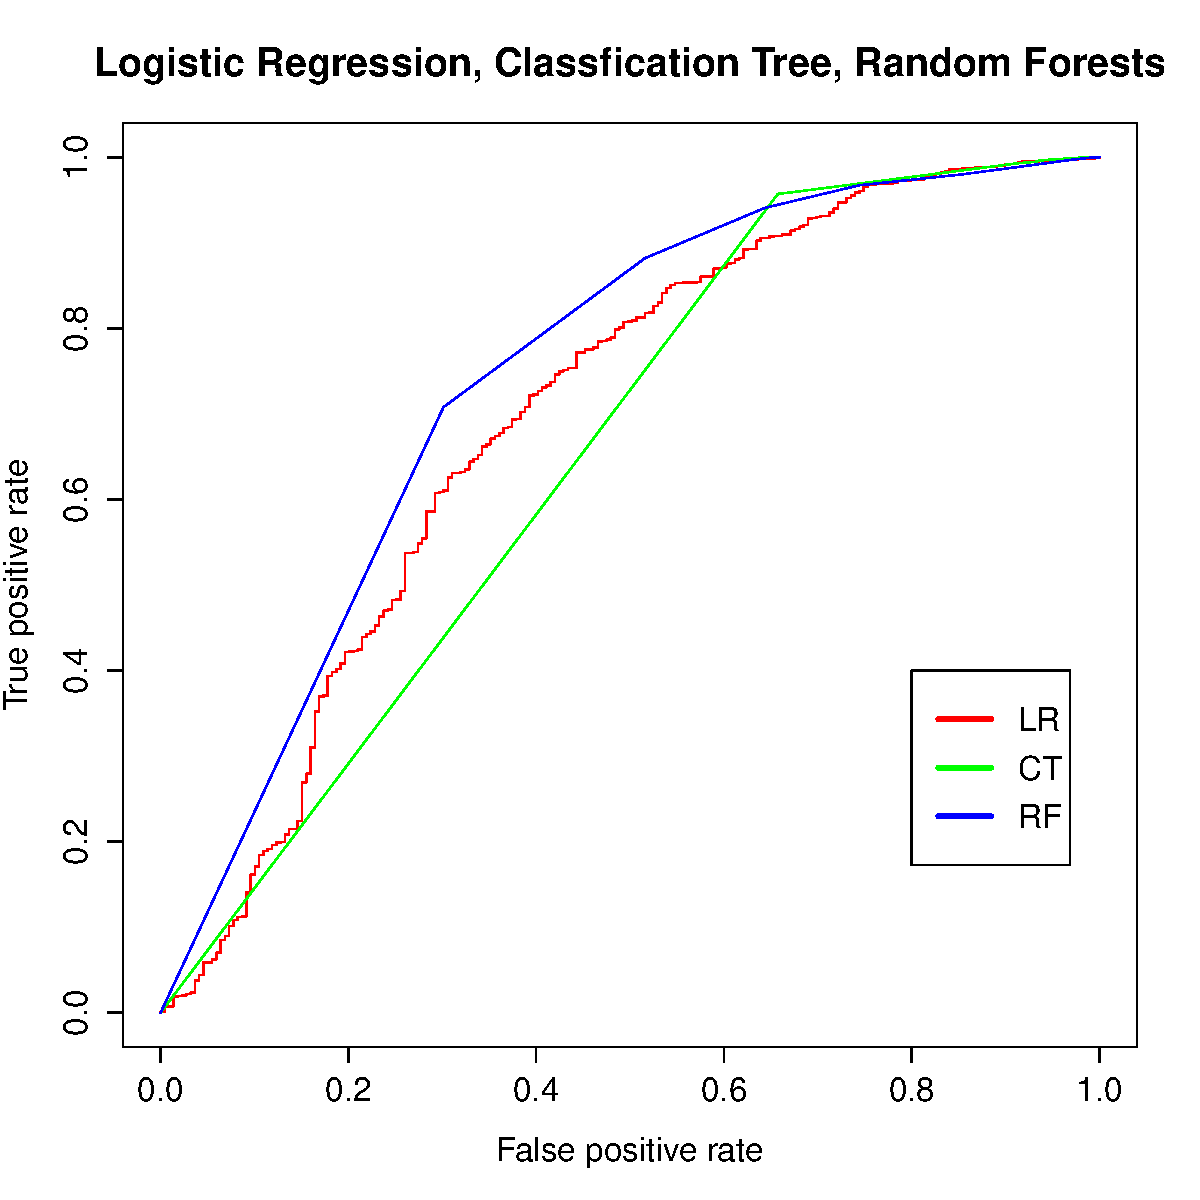
\includegraphics[width=0.8\linewidth]{roc2.pdf}
\caption{\label{fig:roc2}Give Me Some Credit - ROC}
\end{figure}

\begin{table}[htbp]
  \centering
  \caption{Give Me Some Credit}
    \begin{tabular}{lllll}
    \toprule
    Model & KS  & AUC & Accuracy  & Cutoff \\
    \midrule
    LR & 0.329 & 0.695 & 0.933 & 0.727 \\
    CT & 0.300 & 0.651 & 0.933 & 0.308 \\
    RF & 0.407 & 0.741 & 0.932 & 0.300 \\
    \bottomrule
    \end{tabular}%
  \label{tab:roc2}%
\end{table}%
